\item \subquestionpointscodingandwritten{4}
Repeat the steps in part (b) and part (e) for Dataset 2. Create similar plots on
the \textbf{validation set} of Dataset 2 and include those plots in your writeup.

On which dataset does GDA seem to perform worse than logistic regression? Why might this be the case?\\[50pt]

\begin{figure}[H]
    \centering
    \begin{subfigure}{.5\textwidth}
      \centering
      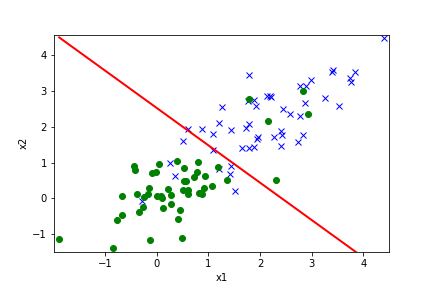
\includegraphics[width=0.95\linewidth]{./linearclass/src/lr_image2.png}
      \caption{Logistic Regression}
    \end{subfigure}%
    \begin{subfigure}{.5\textwidth}
      \centering
      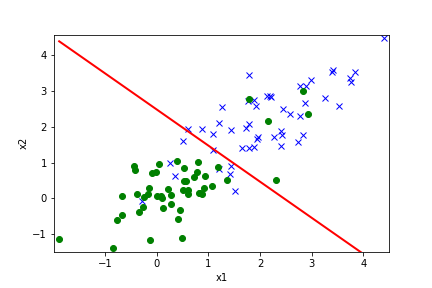
\includegraphics[width=0.95\linewidth]{./linearclass/src/gda_image2.png}
      \caption{GDA}
    \end{subfigure}
    \caption{Dataset 2 Comparison}%
\end{figure}

\hl{GDA performed worse than logistic regression for dataset 1. This is the case because in dataset 1, the data is not Gaussian distributed. GDA performed less well because we made the assumption that the covariance matrix $\Sigma$ was identical for both 0 and 1 labels. From the distribution of the data, we can see that it is not Gaussian distribution and 0 and 1 data points do not have identical $\Sigma$.}
